% !TEX encoding = UTF-8 Unicode
\documentclass[
10pt,
aspectratio=169,
]{beamer}
\setbeamercovered{transparent=10}
\usetheme[
%  showheader,
%  red,
  purple,
%  gray,
%  graytitle,
  colorblocks,
%  noframetitlerule,
]{Verona}

\usepackage[T1]{fontenc}
\usepackage[utf8]{inputenc}
\usepackage{lipsum}
%%%%%%%%%%%%%%%%%%%%%%%%%%%%%%%
% Mac上使用如下命令声明隶书字体,windows也有相关方式,大家可自行修改
%\providecommand{\lishu}{\CJKfamily{zhli}}
%%%%%%%%%%%%%%%%%%%%%%%%%%%%%%%
\usepackage{tikz}
\usetikzlibrary{fadings}
\usetikzlibrary{shapes.geometric}
\usetikzlibrary{positioning}
%\tikzset{
%  every overlay node/.style={
%    draw=black,fill=white,rounded corners,anchor=south west,
%  },
%}
% Usage:
% \tikzoverlay at (-1cm,-5cm) {content};
% or
% \tikzoverlay[text width=5cm] at (-1cm,-5cm) {content};
%\def\tikzoverlay{%
%   \tikz[baseline,overlay]\node[every overlay node]
%}%
\tikzset{
  every overlay node/.style={
    anchor=north west,
  },
}
\def\tikzoverlay{%
   \tikz[baseline,overlay]\node[every overlay node]
}%


\newenvironment{smallgreentext}{\scriptsize\color{green}}{\par}
\newenvironment{smallbluetext}{\scriptsize\color{blue}}{\par}
\def\checkmark{\tikz\fill[scale=0.4](0,.35) -- (.25,0) -- (1,.7) -- (.25,.15) -- cycle;}

%
%\setbeamertemplate{sections/subsections in toc}[ball]
%\usepackage{xeCJK}
\usepackage{adjustbox} % Shrink stuff
\usepackage{listings}
\usepackage{caption}
\usepackage{subcaption}
\usefonttheme{professionalfonts}
\def\mathfamilydefault{\rmdefault}
\usepackage{amsmath}
\usepackage{multirow}
\usepackage{booktabs}
\usepackage{bm}
\setbeamertemplate{section in toc}{\hspace*{1em}\inserttocsectionnumber.~\inserttocsection\par}
\setbeamertemplate{subsection in toc}{\hspace*{2em}\inserttocsectionnumber.\inserttocsubsectionnumber.~\inserttocsubsection\par}
\setbeamerfont{subsection in toc}{size=\small}
\AtBeginSection[]{%
	\begin{frame}%
		\frametitle{Outline}%
		\textbf{\tableofcontents[currentsection]} %
	\end{frame}%
}

\AtBeginSubsection[]{%
	\begin{frame}%
		\frametitle{Outline}%
		\textbf{\tableofcontents[currentsection, currentsubsection]} %
	\end{frame}%
}

\title{Propuesta: Bibliograf\'ia y reporte de originalidad}
\subtitle{Estructuraci\'on y realizaci\'on de la propuesta}
\author[L.M.]{Luis Alejandro Morales, Ph.D.}
\mail{email: lmoralesm@unal.edu.co \\ url: \url{https://lamhydro.github.io}}
\institute[UNAL]{Facultad de Ingenier\'ia, Departamento de Ingenier\'ia Civil y Agr\'icola\\
Universidad Nacional de Colombia, Bogot\'a}
\date{\today}
\titlegraphic[width=3cm]{logo_01u}{}

%%%%%%%%%%%%%%%%%%%%%%%%%%%%%%%%
% ----------- 标题页 ------------
%%%%%%%%%%%%%%%%%%%%%%%%%%%%%%%%
% New commands
\newcommand{\gi}{\texttt{Git}}
\newcommand{\gih}{\texttt{GitHub}}
\newcommand{\co}[1]{\alert{\textbf{\large \texttt{#1}}}}

\begin{document}

\maketitle

%%% define code
\defverbatim[colored]\lstI{
	\begin{lstlisting}[language=C++,basicstyle=\ttfamily,keywordstyle=\color{red}]
	int main() {
	// Define variables at the beginning
	// of the block, as in C:
	CStash intStash, stringStash;
	int i;
	char* cp;
	ifstream in;
	string line;
	[...]
	\end{lstlisting}
}
%%%%%%%%%%%%%%%%%%%%%%%%%%%%%%%%
% ----------- FRAME ------------
%%%%%%%%%%%%%%%%%%%%%%%%%%%%%%%%

%----
\section{Bibliograf\'ia}
\begin{frame}{Bibliograf\'ia}
\begin{block}{Definici\'on}
Una bibliografía es una lista de libros y otros materiales fuente que ha utilizado para preparar un trabajo de investigación. A veces, estas listas incluirán obras que usted consultó pero que no citó específicamente en su tarea. Consulte la guía de estilo requerida para su tarea para determinar el título específico de su página de bibliografía y cómo citar cada tipo de fuente. Las bibliografías generalmente se colocan al final de su trabajo de investigación.
\end{block}
\end{frame}

\begin{frame}{Formatos de Bibliograf\'ia}
\begin{itemize}
\item American Psychological Association (\alert{APA}) style
%\centering
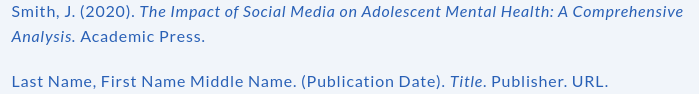
\includegraphics[width=\textwidth]{apa.png}
\item Modern Language Association (\alert{MLA}) style
%\centering

\includegraphics[width=\textwidth]{mla.png}
\item \alert{Chicago} style of citation 
%\centering
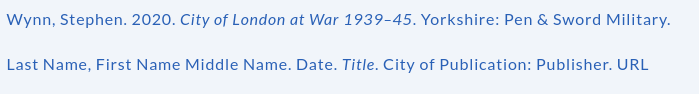
\includegraphics[width=\textwidth]{chi.png}
\end{itemize}
\end{frame}

\begin{frame}{Informacion en la Bibliograf\'ia}
Para articulos, libros, tesis, etc
\begin{itemize}
\item El nombre del autor que estás citando.
\item El título de la publicación que estás citando.
\item Título del artículo (si se utiliza un artículo de revista o revista).
\item El número de volumen de la revista, revista o enciclopedia que cita, o la edición que cita en el caso de una publicación impresa.
\item Fecha de publicación.
\item Lugar de publicacion.
\item Editor.
\item Número(s) de página relevantes para su investigación y que está citando en su trabajo.
\end{itemize}
\end{frame}

\begin{frame}{Informacion en la Bibliograf\'ia}
Pagina web y recursos en internet
\begin{itemize}
\item El nombre del autor y/o editor del artículo web que estás citando.
\item  El título del sitio web que estás citando.
\item  Empresa u organización propietaria del sitio web o que publica en él.
\item  URL (dirección del sitio web).
\item La fecha en que accedió a la información que está citando y, cuando sea posible, la fecha en que se publicó originalmente la información que está citando.
\end{itemize}
\end{frame}

\begin{frame}{¿Como citar?}
\begin{itemize}
\item Citas entre parentesis
Para las citas entre paréntesis, tanto el autor como la fecha aparecen separados por una coma. Una cita entre paréntesis puede aparecer dentro o al final de una oración. E.g. \textbf{...98\% of participants \alert{(Smith, 2014)}}
\item Citas narrativas
En las citas narrativas, el apellido del autor aparece en el texto corriente mientras que la fecha aparece entre paréntesis después. El nombre del autor se puede colocar en cualquier parte de la oración que tenga sentido. E.g. \textbf{\alert{Yang (2004)} suggested that...}
\end{itemize}
\end{frame}

\section{Reporte de originalidad}
\begin{frame}{Formas de plagio}
\begin{itemize}
\item Cita textual (palabra por palabra) sin reconocimiento claro
\item Parafrasear
\item Colusi\'on
\item Cita inexacta
\item Falta de reconocimiento de asistencia por parte de otros
\item Uso de material escrito por agencias profesionales u otras personas
\item Autoplagio
\end{itemize}
\end{frame}

\begin{frame}{Reporte de originalidad: Turnitin}
\begin{itemize}
\item Verifica la similitud en los trabajos escritos
\item Enseña la importancia del trabajo original
\item Compara los trabajos de los estudiantes con la base de datos más completa del sector.
\item Revisa el porcentaje de similitud de una tarea, obtén resultados codificados por colores y compara con las fuentes.
\end{itemize}
\end{frame}

\end{document}
